
% --- OVO MORA BITI OVDE, UNUTAR DOKUMENTA ---
% Ovim komandama nasilno menjamo engleske nazive u srpske
% jer ih stavljamo nakon što se učitala klasa.
\renewcommand{\figurename}{Slika}
\renewcommand{\tablename}{Tabela}
\renewcommand{\proofname}{Dokaz}
\renewcommand{\abstractname}{Sažetak}
\renewcommand{\refname}{Literatura}
% -------------------------------------------


\Author{Kosta Mašulović, Simon Savić}
\Title{Kompaktna popločavanja L-trominama}
\TitleEng{Fault-free L-tromino tillings}
\begin{Abstract}

U ovom projektu bavili smo se kompaktnim popločavanjima i popunjavanjima L-trominama, kako u dvodimenzionalnim i trodimenzionalnim, tako i u višedimenzionim prostorima. Kompaktno popločavanje pravougaonika je poznat princip, ali sta se dešava ako želimo da popločamo neko složenije telo, kao na primer cilindar? Naime, kada se površno pogleda izgleda kao da je analogna stvar, jer je isto kao i pravougaonik, ali ako se spoji u omotač uviđa se problem nekompaktnosti takvog popločavanja, što ukazuje na to da se mora osmisliti neki novi način. Još jedno pitanje koje se nameće jeste, šta se dešava u višedimenzionom prostoru i da li je moguće nekako izvesti ideju kompaktnosti iz 2D. Problem kod ovoga jeste, kako zamisliti trominu u takvim prostorima i šta tu predstavlja kompaktno popločavanje, odnosno, popunjavanje. 

\end{Abstract}
\begin{AuthorEx}
Kosta Mašulović (2006), Novi Sad, 3. razred, Gimnazija ‚‚Jovan Jovanović Zmaj", Novi Sad
\newline
\newline
Simon Savić (2006), Čurug, 3. razred, Gimnazija ‚‚Jovan Jovanović Zmaj", Novi Sad
\newline
\newline
MENTORI:
\newline
Prof. dr Bojan Bašić, Prirodno-matematički fakultet, Univerzitet u Novom Sadu
\newline
\newline
Aleksa Džuklevski, Prirodno-matematički fakultet, Univerzitet u Novom Sadu
\end{AuthorEx}
\begin{AbstractEng}
In this paper, we investigate the problem of fault-free tilings with L-trominoes across two-dimensional, three-dimensional, and higher-dimensional spaces. An L-tromino is defined as a polyomino consisting of three unit squares arranged in an L configuration, while a tiling is deemed fault-free if no horizontal or vertical line can traverse the tiled body without intersecting at least one tile. Although fault-free tilings of rectangles are well established, the question arises as to what occurs when one attempts to tile more complex bodies.
We present explicit constructions of fault-free tilings for two-dimensional manifolds including the cylinder, Möbius strip, and torus. In three dimensions, we establish that any cuboid with at least one side length divisible by three admits to a fault-free tiling with three-dimensional L-trominoes. This result is obtained by reducing the problem to the two-dimensional case and applying known theorems on compact tilings of rectangles. Extending the framework further, we introduce the notion of higher-dimensional L-trominoes and fault-free tilings in such spaces. Through dimensional reduction and the principle of mathematical induction, we prove that any hypercuboid with at least one dimension divisible by three can be tiled in a fault-free way with higher-dimensional L-trominoes.
At the very end of this paper, we derive a lower bound for the number of distinct fault-free tilings of a three-dimensional cuboid.



\end{AbstractEng}
\StartDoublePaper
\label{doc:rad}

\AuthorExHere
\section{Uvod}

L-tromina kao pojam s kojim su svi upoznati, može se zamisliti kao figura sastavljena od tri jedinična kvadrata spojena tako da formiraju slovo "L". Posle domina, to je jedna od najpoznatijih figura koja se koriste za popločavanje. Generalno gledano, na popločavanje trominama matematičari su prešli kada su sa dominama već dokazali većinu stvari. Danas se zna koji se sve to kvadrati i pravougaonici mogu kompaktno popločati, tj. koji su uslovi za to. Međutim, nije poznato kako se ponašaju neki drugi oblici poput cilindra i njemu sličnih tela što nas je dovelo do prvog cilja i izvora problema. Naravno, to smo znali da neće biti nešto preterano izazovno. Nas je pre svega najviše zaintrigiralo to što za 3D popločavanje nije bilo ništa poznato, pa smo bili najpre vođeni tom rupom u istraživanju popločavanja. Dok smo rešavali problem popločavanja omotača kvadra, dobili smo ideju da definišemo potpuno nov koncept, kompaktnog popunjavanja, koji smo definisali kao analogan pojam kompaktnom popločavanju, samo u 3D. Tako smo imali motiv da i mi nađemo uslov koji treba da ispuni kvadra da bi ga bilo moguće popuniti i ovo nam je bio prvi veliki izazov. Prilikom rešavanja ovog izazova zapitali smo se: Šta ako ovaj princip proširimo na sve dimenzije? I tako smo započeli problem prikazivanja L-tromina u višedimenzionim prostorima, započinjući u 4D, gde smo uvideli princip koji se ponavlja i vođeni time smo uspeli da konstruišemo teoremu koja govori o univerzalnom popunjavanju u nD.
Kroz naše istraživanje, uspeli smo da formulišemo teoremu koja osvetljava uslove potrebne za postizanje kompaktnih popunjavanja kvadra L-trominima u trodimenzionalnom i višedimenzionalnom prostoru. Ova teorema ne samo da doprinosi razumevanju višedimenzionalnog popločavanja, već otvara i nova pitanja i izazove za buduća istraživanja. Kroz ovo istraživanje, obogatili smo naše znanje o trominama, popločavanjima, ali smo stvorili i 
temelje za dalje analize u oblasti popločavanja i kombinatorne geometrije. Naš rad predstavlja korak napred u razumevanju i primeni koncepta popločavanja u višim dimenzijama, pružajući nova saznanja i mogućnosti za istraživanje u ovom uzbudljivom polju matematike.


\section{Uvodni pojmovi i korisne teoreme}

U ovoj sekciji biće definisani osnovni pojmovi i tvrđenja koji će se koristiti u daljem radu. Pre svega, čitalac mora biti upućen da je poliomina geometrijska figura formirana spajanjem jednog ili više jednakih kvadrata po ivicama. Budići da je fokus rada zasnovan na L-trominama, po definiciji iz knjige ‚‚Polyominoes" [3], L-tromina se definiše preko poliomina na sledeći način. 

\begin{Definition}
       Za poliominu se kaže da je L-oblika ako ima 6 temena. Po definiciji [3], poliomine L-oblika se definišu kao $L(a, b, c)$, gde $a$ i $b$ predstavljaju dužinu L-poliomine, a $c$ jediničnu visinu svakog sprata kao što je prikazano na slici 1.
\end{Definition}

Analogno se iz definicije 2.1 definiše L-tromina.

\begin{Definition}
    L-tromina je poliomina L-oblika za koju važi $L(1, 2, 1)$.  
\end{Definition}

Za potrebe daljeg rada u višedimenzionom prostoru, definisaće se L-tromina u višim dimenzijama.

\begin{Definition}
      n-dimenziona L-tromina je L-tromina kojoj je dodato $n$ dimenzija jedinične vrednosti.
\end{Definition}

Žargonski rečeno, radi korišćenja L-tromine u određenoj dimenziji, ona će se ”izdići” za jediničnu vrednost po dimenziji normalnoj na sve ostale dimenzije L-tromine.

U prvom planu rada nalazi se kompaktno popločavanje figura, stoga je neophodno definisati kompaktno popločavanje. Klasično popločavanje po svojoj prirodi predstavlja pokrivanje površine, najčešće ravni, koristeći jedan ili više geometrijskih oblika, zvanih pločice, bez preklapanja i praznina.

\begin{Definition}
    Kompaktno popločavanje figure je popločavanje u kojem nije moguće povući pravu (horizontalnu ili vertikalnu) koja prolazi kroz popločanu figuru tako da nijedna pločica u figuri ne bude presečena tom pravom.
\end{Definition}

Kao što je već navedeno, u radu biće takođe reč i o višedimenzionom popločavanju, to jest kompaktnom popunjavanju figura. Popunjavanje tela je popunjavanje zapremine nekog tela drugim unapredzadatim telima. Kao i kod popločavanja, kod popunjavanja nije dozvoljeno ostaviti bilo koji deo zapremine nepopunjen, odnosno, žargonski rečeno, rupe nisu dozvoljene.

\begin{Definition}
    Kompaktno popunjavanje nekog tela je popunjavanje u kojem nije moguće naći ravan koja preseca to telo tako da nijedna figura unutar njega ne bude presečena.
\end{Definition}

Imajući u vidu kompaktno popločavanje, do sada su poznata popločavanja određenih pravougaonika [3]. Ove osobine će se koristiti u daljem radu za dokazivanje problema u višedimenzionim prostorima.  

\begin{Theorem}
    Neka je $1\leq m<n $ i (m,n)=1. Tada se pravougaonik p,q može kompaktno popločati ako i samo ako važi:
    \begin{enumerate}
        \item I m i n dele p ili q
        \item I p i q se mogu izraziti kao xm+yn na bar dva različita načina gde $x,y>0$
        \item za m=1 i n=2 , $p,q\neq6$
    \end{enumerate}
\end{Theorem}

Poznato je da svi pravougaonici koji se mogu popločati pravougaonicima $3\times2$ se takođe mogu i kompaktno popločati određenim rasporedom L-tromina [3]. Moguće je kompaktno popločati i pojedine pravougaonike koji se ne mogu popločati $3\times2$ pravougaonicimo, no ovo su vrlo specfični slučajevi te se mogu pronaći u literaturi [3]. Ovo tvrđenje se može uopštiti  i koristiće se u daljem dokazivanju.

\begin{Theorem}
    Svi p×q pravougaonici gde važi $p,q \geq 4$ i $3\mid pq$, mogu se kompaktno popločati L-trominama.
\end{Theorem}


\section{Rešenja u 2D}

Istorijski posmatrano, svi problemi vezani za tematiku poliomina  su rešavani u dvodimenzionalnim prostorima. Budući da su svi problemi koji se odnose na kompaktno popločavanje pravougaonika rešeni ili pak nisu dovoljno interesantni za bilo kakvo unapređenje, odlučili smo se za kompaktno popločavanje tela koja u svrhu postizanja željenog rezultata koriste drugačije pristupe rešavanju problema. 

Prvi rezultati u ovom radu zasnovani su na kompaktnom popločavanju trodimenzionih tela, tačnije njihovih omotača koja se svode na popločavanje površi svedenih u dvodimemzioni prostor. Iako se ove površi nalaze u trodimenzionalnom prostoru, površi kao takve zadržavaju svoja svojstva, to jest poseduju samo dve dimenzije pozitivnih vrednosti. Samim tim, ispravnim razvićem i smeštanjem u ravan, kompaktno popločavanje ovih površi se može pokušati svesti na neki dosada već rešen problem uz male ispravke.

Naime, svi oblici korišćeni u dosadašnjoj literaturi bili su konveksni oblici sačinjeni od jediničnih kvadrata (pravougaonici različitih dimenzija). Kako bi popločavanja ovih površi bila kompaktna, potrebno je razviti površi na način koji za rezultat neće dati konveksan oblik. Ovaj korak je od krucijalne važnosti zbog uslova kompaktnog popločavanja. Ako uzmemo cilindar kao primer, očigledno je da njegovo najintuitivnije razviće za rezutat daje pravougaonik. Ponovnim konstruisanjem cilindra od dobijenog pravougaonika daje cilindar koji nije kompaktno popločan budući da dva spojena kraja obrazuju duž po kojoj je moguć rez bez presecanja ijedne tromine. Dakle, potrebno je razviti figuru na način koji je nekonveksan i da krajevi te figure poseduju ‚‚šiljke" koji bi se međusobno uklapali. ‚‚Šiljci", to jest delovi koji čine figuru nekonveksnom će su u procesu sastavljanja figure međusobno uklapati, spajajući krajeve tih figura i činiti ih kompaktno popločanim.

Dvodimenzionalne površi smeštene u trodimenzionalni prostor čija kompaktna polpočavanja će biti ispitivana u ovom radu su cilindar, Mebijusova traka i torus.

\subsection{Cilindar}
Cilindar, kao jednostavno geometrijsko telo čiji omotač predstavlja dvodimenzionu površ smeštenu u trodimenzionom prostoru, bio je pogodan model za razvoj intuicije u vezi sa kompaktnim popločavanjem. U našem pristupu, omotač cilindra je razvijen u pravougaonik radi pojednostavljene analize popločavanja. Konkretno, fokusirali smo se na slučaj cilindra minimalne složenosti, pri čemu je vrednost dimenzije duž $y$ ose minimalna. Rezultat ovog kompaktnog popločavanja predstavljen je na slici 1.


%\begin{figure}
 %   \centering
  %  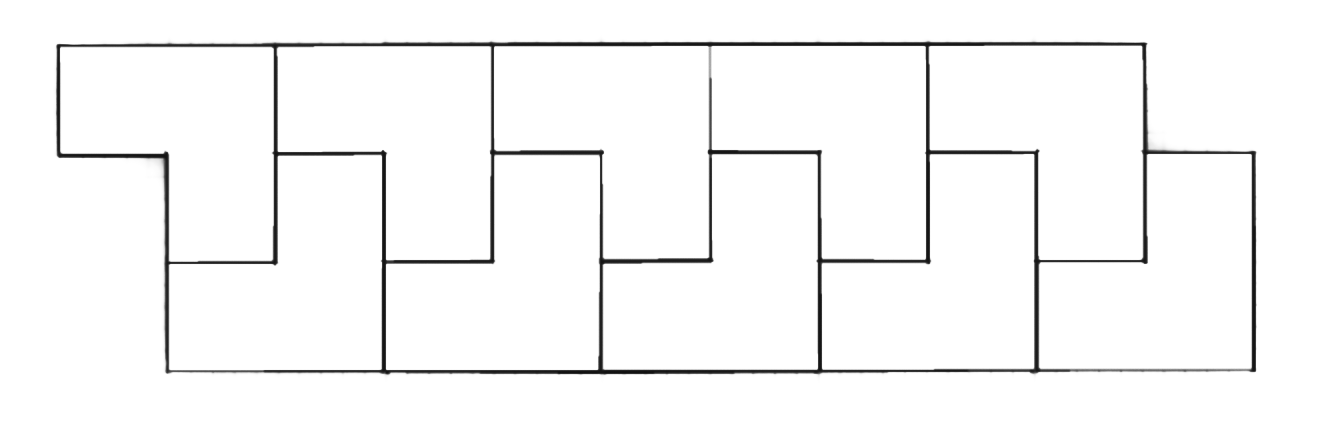
\includegraphics[width=7cm]{cilindar1.png}
   % \caption{Kompaktno popločavanje cilindra.} 
%\end{figure}

\Figure{cilindar1.png}{Kompaktno popločavanje cilindra}{Compact tiling of the cylinder}
Budući da je cilindar kao problem isključivo predstavljao ‚‚zagrevanje", nismo razmatrali mogućnosti složenijeg kompaktnog popločavanja, to jest kompaktnog popločavanja cilindra većih dimenzija.

\subsection{Mebijusova traka}

Naredna kopmaktno popločana površ je Mebijusova traka. Budući da je Mebijusova traku moguće izvesti iz cilindra rotiranjem jedne stranice i spajanjem sa nerotiranom stranicom na suprotnoj strani pravougaonika, intuicija navodi na svođenje problema na problem kompaktnog popločavanja cilindra. Mebijusova traka za razliku od cilindra se ‚‚uvrće" i samim time potrebno je da su gornji i donji delovi jednog kraja simetrični u odnosu na $x$ osu ili pak da su L-tromine lukavo raspšoređene tako da se uklapaju pri spajanju krajeva. Jedan primer kompaktno popločane Mebijusove trake dat je na Slici 2.

%\begin{figure}[!h]
 %   \centering
 %   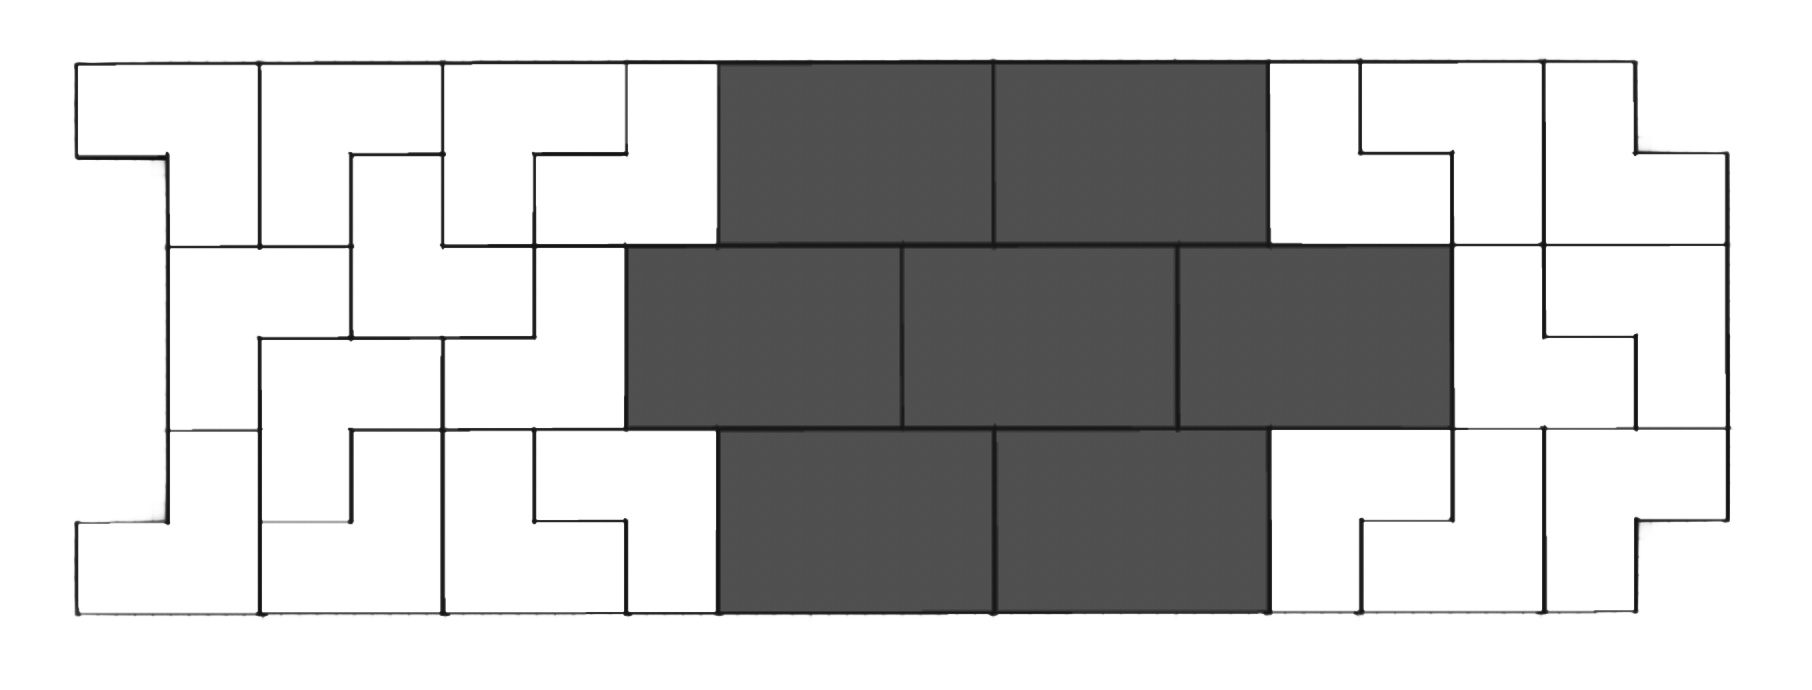
\includegraphics[width=7cm]{MT1.png}
  %  \caption{Kompaktno popločavanje Mebijusove trake.} 
%\end{figure}
\Figure{MT1.png}{Kompaktno popločavanje Mebijusove trake}{Compact tiling of the Möbius strip}
Mebijusova traka se može širiti i po $x$ i po $y$ osi. Po $x$ osi Mebijusova traka se ‚‚produžava" pomoću osenčenih pravougaonika. Ređanjem osenčenih pravougaonika po $x$ u na slici datoj konfiguraciji nam omogućava produžavanje trake u beskonačnost. Raspored osenčenih pravougaonika je izbran radi ispunjavanja uslova kopaktnog popločavanja, dok sami pravouganici predstavljaju parove međusobno spojenih L-tromina [3].

Po $y$ osi Mebijusova traka se produžava pomoću konfiguracije na Slici 3. Produžavanje se vrši tako što se dve Mebijusove trake konfiguracije sa Slike 2 slažu jedna na drugu tako da dva osenčena pravougaonka sa prve i dva osenčena pravougaonika sa druge obrazuju konfiguraciju sa Slike 3. Ova konfiguracija omogućava ispunjenje uslova kompaktnog popločavanja. Ovaj način produžavanja se može vršiti u ezbroj iteracija, samim time omogućavajući peskonačno produžavanje Mebijusove trake po $y$ osi.

%\begin{figure}[!h]
 %   \centering
  %  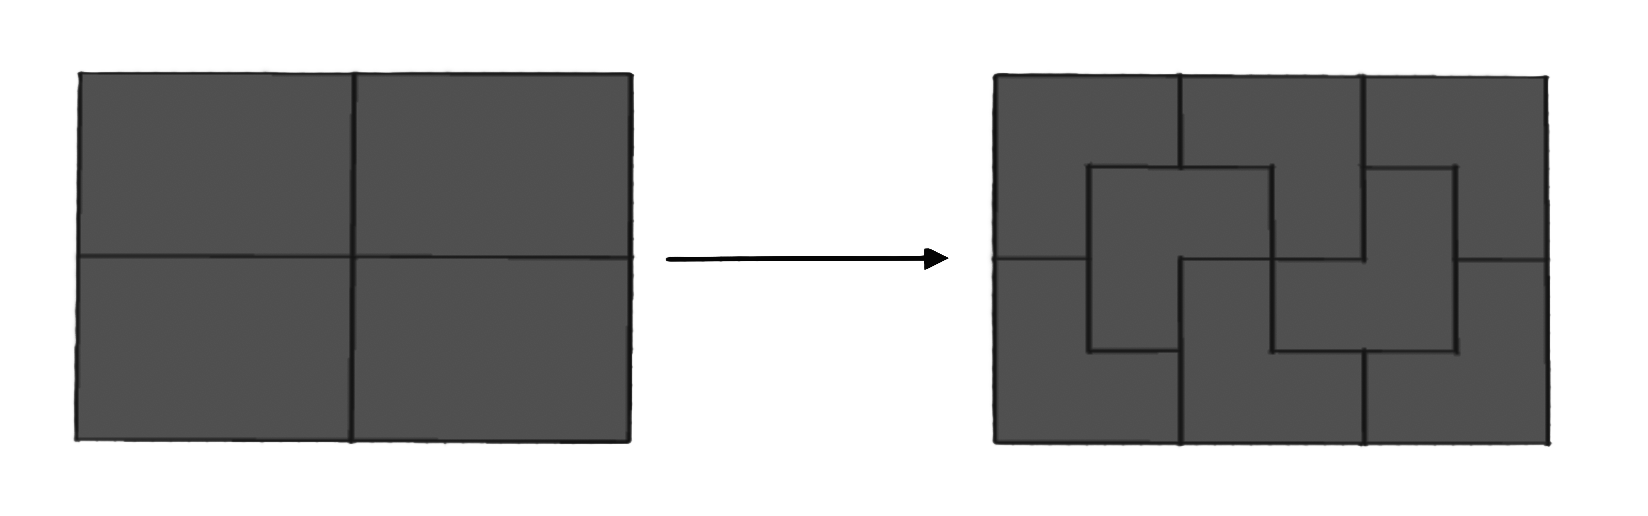
\includegraphics[width=7cm]{A1}
   % \caption{Konfiguracija korištena za osobine Mebijusove trake i torusa.} 
%\end{figure}
\Figure{A1.png}{Konfiguracija korištena za osobine Mebijusove trake i torusa}{Configuration used for the properties of the Möbius strip and the torus}

\subsection{Torus}

Poslednja i ubedljivo najkomplikovanija kompaktno popločana površ je torus. Rešenje za torus se direktno izvodi iz rešenja Mebijusove trake. Za razliku od mebijusove trake gde se samo levi i desni kraj spajaju, kod torusa pored levog i desnog kraja se takođe spajaju i gornji i donji kraj. Osobina kompaktnog popločavanja nameće problem modifikacije rasporeda L-tromina koje spajaju gornju i donju stranu razvijenog torusa. Važenje osobina se zadovoljava primenom konfiguracije sa slike 3 na gornja i donja dva osenčena pravougaonika Mebijusove trake. Primenjivanjem ove konfiguracije dobija se razvijen kompaktno popločan torus sa slike 4.


%\begin{figure}[!h]
 %   \centering
  %  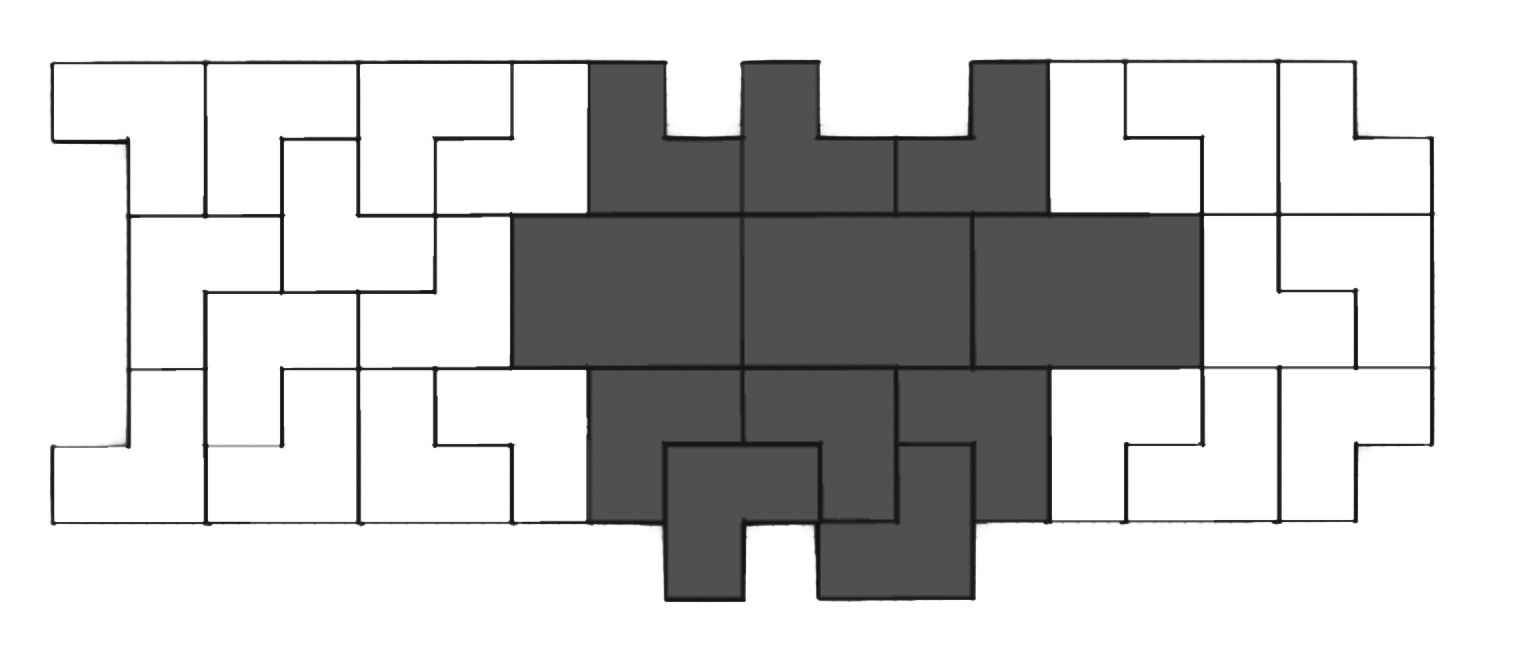
\includegraphics[width=7cm]{Torus1.png}
   % \caption{Kompaktno popločavanje torusa.} 
%\end{figure}
\Figure{Torus1.png}{Kompaktno popločavanje torusa}{Compact tiling of the torus}

Kao i kod Mebijusove trake, povećavanje dimenzija po obe ose kordinatnog sistema je moguć po istom principu.


\section{Rešenja u 3D}

Nakon analize kompaktnog popločavanja dvodimenzionalnih površi, pažnja je usmerena na trodimenzionalna tela, pri čemu su razmatrani isključivo kvadri. U trodimenzionom prostoru razlikuju se dva pristupa popločavanju: prvi se odnosi na kompaktno popločavanje omotača kvadra, dok drugi obuhvata kompaktno popunjavanje njegove zapremine. Radi preciznosti, u daljem tekstu, kada se govori o kompaktnom popločavanju omotača, misli se isključivo na površ kvadra, dok se u svim ostalim slučajevima podrazumeva kompaktno popunjavanje zapremine.

U nastavku, razmatra se generalizacija ovih ideja na više dimenzije, sa fokusom na principe kompaktnog popunjavanja u višedimenzionim prostorima.






Budući da se posmatra kompaktno popunjavanje prostora u tri dimenzije, neophodno je da i strukture korišćene za popunjavanje pripadaju trodimenzionalnom prostoru.Uzimajući ovo u obzir, pojam $L$-tromine u trodimenzionalnom prostoru definiše se kao proširenje odgovarajuće definicije iz dvodimenzionog prostora.
\begin{Definition}
    $L$-tromina u trodimenzionom prostoru je telo sastavljeno od jediničnih kocki spojenih po ivicama tako da dobijeno telo ima 12 temena.
\end{Definition}

\begin{Theorem}
    Svaki kvadar $p×q×r$ gde važi $p,q \geq 4$ i $3\mid pqr$, može se kompaktno popločati trodimenzionalnim L-trominama.
\end{Theorem}
Za potrebe dokaza ove teoreme definišemo pojam kritične tromine, kao i pomoćnu lemu koja govori o broju tromina koje nisu kritične.

\begin{Definition}
    Kritična tromina je tromina koja sprečava neku od pravih(ravni) da preseku figuru tj. tromina bez koje telo ne bi bilo kompaktno popločano(popunjeno).
\end{Definition}




\begin{Proof}
    Kvadar se deli na slojeve jedinične visine i svaki sloj se popločava zasebno. Kako su ti slojevi pravougaonici dimenzija $p\times q$ izdignuti za jednu jedinicu, za njih je poznato po teoremi 2.7 da se mogu kompaktno poplocati ako je $p,q \geq 4$ i $3\mid pq$.
    Da bi kvadar bio kompaktno popunjen iz uslova kompaktnosti sledi da susedni slojevi moraju biti medjusobno povezani, tacnije mora se pojaviti bar jedna kriticna tromina koja ih povezuje.Ta kriticna tromina bice formirana tako sto će se izabrati bilo koja tromina koja nije kritična u tom sloju i koja je u tom sloju u potpunosti i rotira se za 90 stepeni u smeru ka gornjem sloju tako da 2 jedinične kocke koje sacinjavaju tu trominu ostanu u tom sloju. Tom rotacijom pravi se praznina u donjem sloju ekvivalentan jediničnoj kocki. Da bi se ta praznina popunila na analogan način ćemo rotirati L-trominu koja se nalazila direktno iznad već rotirane tromine tako da ona popuni prazninu donjeg sloja.(Slika 5)
    Kako znamo da uvek mžemo da izaberemo trominu koja će postati kritična to znači da možemo spojiti bilo koji broj slojeva međusobno, što znači da ta dimenzija ne utiče na to da li se kvadar može kompaktno popuniti, a i samim tim da je jedini uslov koji je potreban da bi se kvadar mogao kompaktno popuniti da mu je bar jedna dimenzija deljiva sa 3, čime je dokaz gotov.
\end{Proof}




%\begin{figure}[!h]
 %   \centering
  %  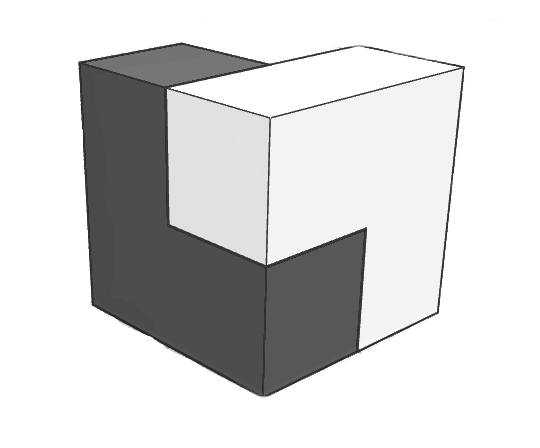
\includegraphics[width=5cm]{K1.png}
   % \caption{Spajajuća konfiguracija sačinjena od dve tromine.} 
%\end{figure}
\Figure{K1.png}{Spajajuća konfiguracija sačinjena od dve tromine}{Connecting configuration composed of two trominoes}

Primeri rasporeda tromina u dvodimenzionalnoj formi slojeva predstavljeni su na Slikama 6 i 7 gde $D$ označava donji, dok $G$ gornji sloj. Sopstvenom bojom su osenčene tromine, gde jedna boja predstavlja izdignutu trominu u oba sloja. Šrafiran deo predstavlja proizvoljan raspored L-tromina po Teoremi 2.7, dok su koordinate jediničnih kocki date radi lakšeg sticanja intuicije za spajanje slojeva.


%\begin{figure}[!h]
 %   \centering
  %  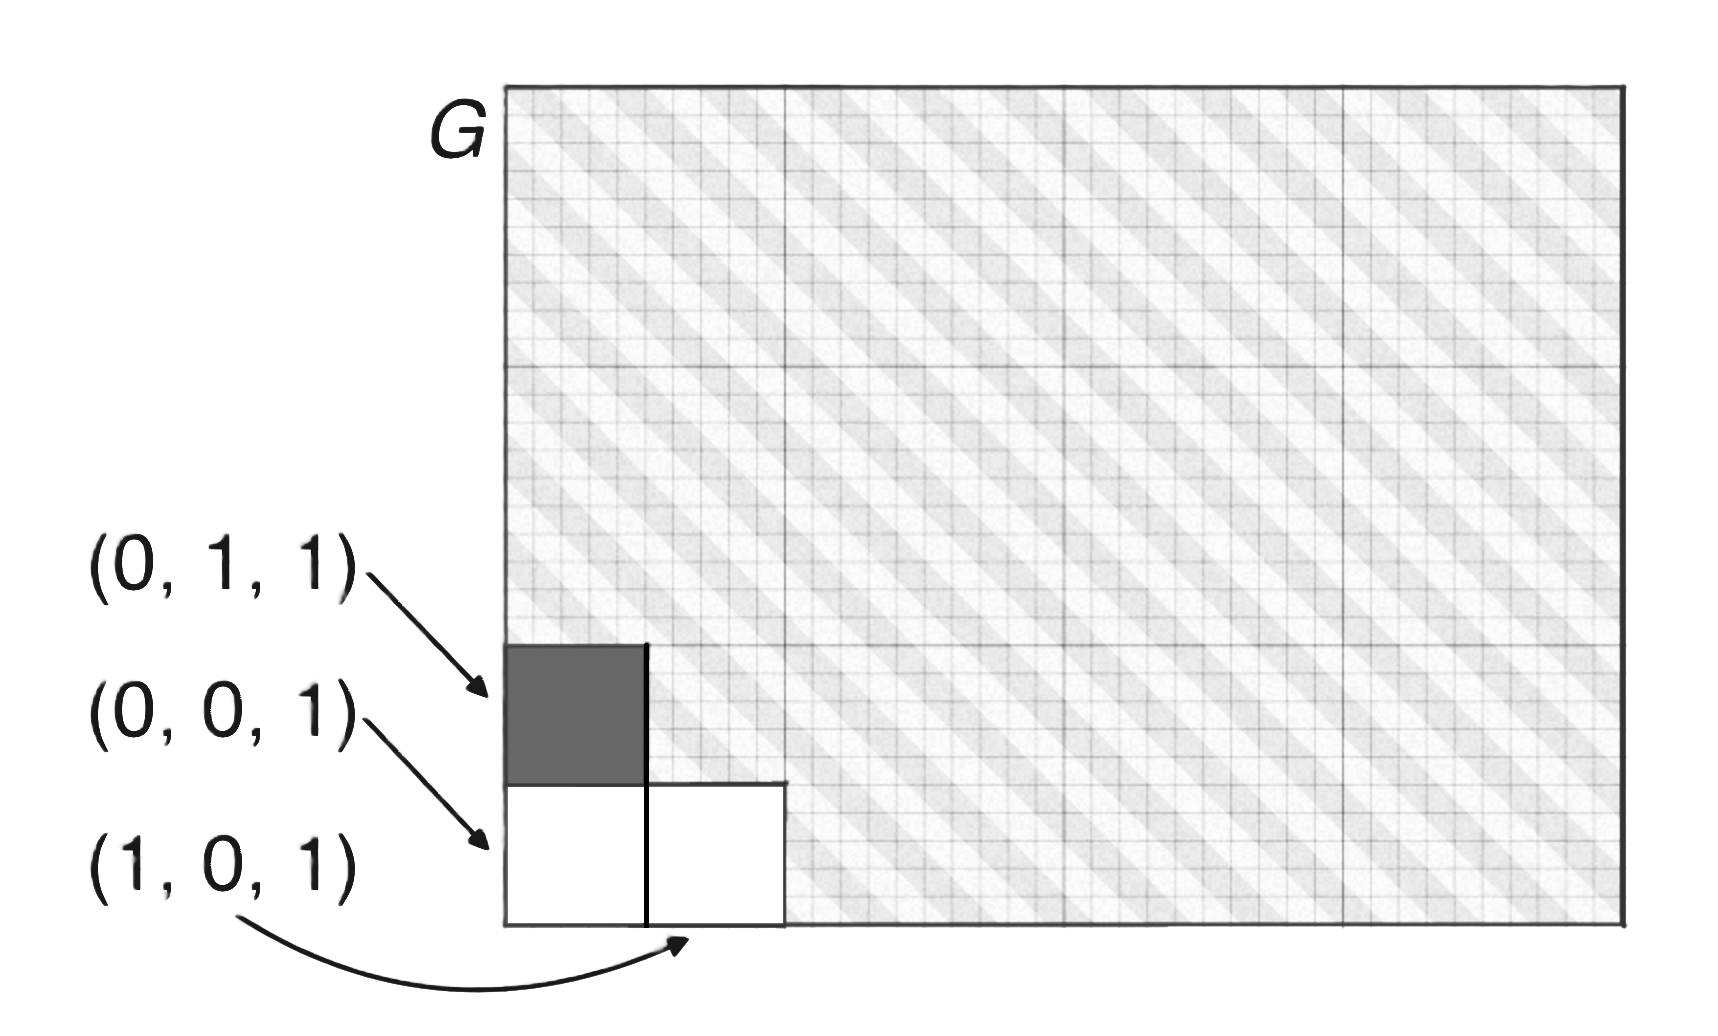
\includegraphics[width=7cm]{3D-G(1).png}
   % \caption{Dvodimenzionalna forma gornjeg sloja.} 
%\end{figure}
\Figure{3D-G(1).png}{Dvodimenzionalna forma gornjeg sloja}{Two-dimensional form of the upper layer}

%\begin{figure}[!h]
 %   \centering
  %  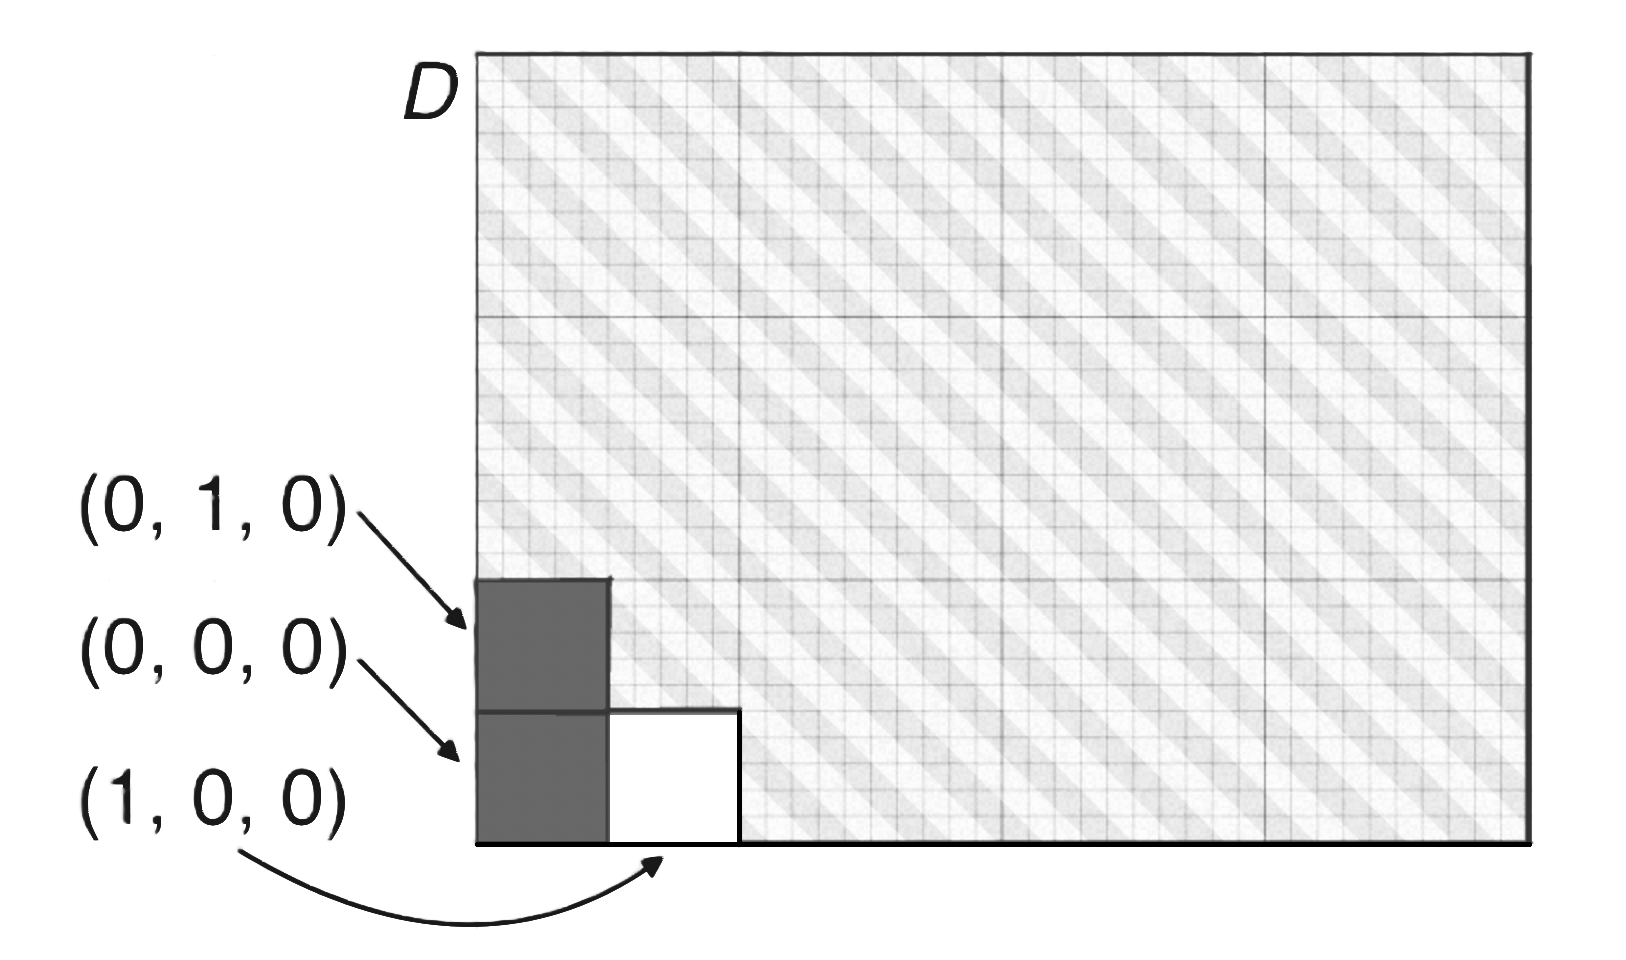
\includegraphics[width=7cm]{3D-D(1).png}
   % \caption{Dvodimenzionalna forma donjeg sloja.} 
%\end{figure}
\Figure{3D-D(1).png}{Dvodimenzionalna forma donjeg sloja}{Two-dimensional form of the bottom layer} 

\section{Rešenje u nD}
%Nastavljajući sa radom, prešli smo u sledeće dimenzije, gde smo se bavili problematikom prikazivanja tromina i kompaktnog popunjavanja u 4D i nakon toga smo dobili naš najveći rezultat, tj. osmislili smo teoremu koja govori o kompaktnom popunjavanju kvadrova u nD, a čiji se dokaz izvodi induktivno.

Nakon dokazivanja kompaktnog popunjavanja kvadra, prirodno je postaviti pitanje može li se kompaktno popuniti višedimenzioni kvadar? Rezon je sličan kao i kod trodimenzionog kvarda sa par izmena. Ispostavlja se da je rešenje višedimenzionog kompaktnog popunjavanja izvedeno iz dokaza kompaktnog popunjavanja trodimenzionog kvadra, što navodi na dokaz matematičkom indukcijom.

%Nastavljajući sa radom, prešli smo na dokazivanje istog problema za četvorodimenzioni kvadar. Rezon je sličan kao i kod trodimenzionog kvarda sa par izmena. Ispostavilo se da je način dokazivanjna izveden iz dokaza trodimenzionog kvadra što navodi na dokaz kompaktnog popločavanja n-dimenzionog kvadra zasnovan na matematičkoj indukciji.

\begin{Theorem}
    Svaki kvadar $p\times q\times r\times s$ za koji važi $p,q \geq 4$ i $3\mid pqrs$, može se kompaktno popuniti četvorodimenzionim L-trominama.
\end{Theorem}
Budući da nam je poznat dokaz kompaktnog popunjavanja kvadra,


Dokaz Teoreme 5.1 je sledeći. Budući da je poznat dokaz kompaktnog popunjavanja trodimenzionog kvadra, potrebno je problem kompaktnog popunjavanja četvorodimenzionog kvadra svesti na problem manje dimenzije. Ovo se postiže na sličan način koa kod popunjavanja kvadra. Prvo se četvorodimenzioni kvadar podeli na četvorodimenzione slojeve jedinične četvorodimenzione visine (po $t$ osi - četvrta osa). Zbog jedinične četvorodimenzione visine, dobijeni slojevi se mogu posmatrati kao trodimenzioni objekti. Po teoremi 4.1 ovi slojevi se mogu kompaktno popločati. Kao i kod kompaktnog popunjjavanja trodimenzionog kvadra potrebno je pronaći spajajuću konfiguraciju kako bi dva sloja bila spojena. Radi lakšeg snalaženja u četvorodimenzionom prostoru, tromine ćemo opisati koordinatama. Predstavljanje pomoću koordinata će funkcionisati tako što koordinate jedne tačke predstavljaju jednu kocku L-tromine.

%Kada se slojevi ‚‚izdignu" u četvrtu dimenziju, sa njima će i tromine koje omogućavaju spajajuću konfiguraciju, i budući da se nalaze na istim kordinatama, gde je samo visina promenjena za jednu jedinicu, oformiće spajajuću konfiguraciju u četvrtoj dimenziji.


Kako bi spojili dva sloja, potrebno je da se dve domine na istim mestima u dva sloja zamene trominama u drugačijoj konfiguraciji. Primera radi, ako se u gornjem i donjem sloju izaberu tromina sa sledećim koordinatama: $$T_G\{(a, b+1, c, 1), (a, b, c, 1), (a+1, b, c, 1)\}$$  $$T_D\{(a, b+1, c, 0), (a, b, c, 0), (a+1, b, c, 0)\}$$
Kako bi se postigla spajajuća konfiguracija, potrebno je zameniti date tromine sa trominama sa sledećim koordinatama [Slike 8 i 9]: $$T_1\{(a, b+1, c, 1), (a, b, c, 1), (a, b+1, c, 0)\}$$  $$T_2\{(a+1, b, c, 1), (a, b, c, 0), (a+1, b, c, 0)\}$$ Primetimo da se nakon zamene tromine istovremeno nalaze u dva odvojena sloja. Budući da su slojevi zapravo četvorodienzioni oblici koji su zbog jedinične četvorodimenzione visine predstavljeni kao trodimenzione figure, kada se slojevi spoje u četvrtoj dimenziji, zajedno sa njima ce i tromine koje formiraju spajajuću konfiguraciju postati četvorodimenzione spajajući dva sloja četvorodimenzionog kvadra.


%\begin{figure}[!h]
 %   \centering
  %  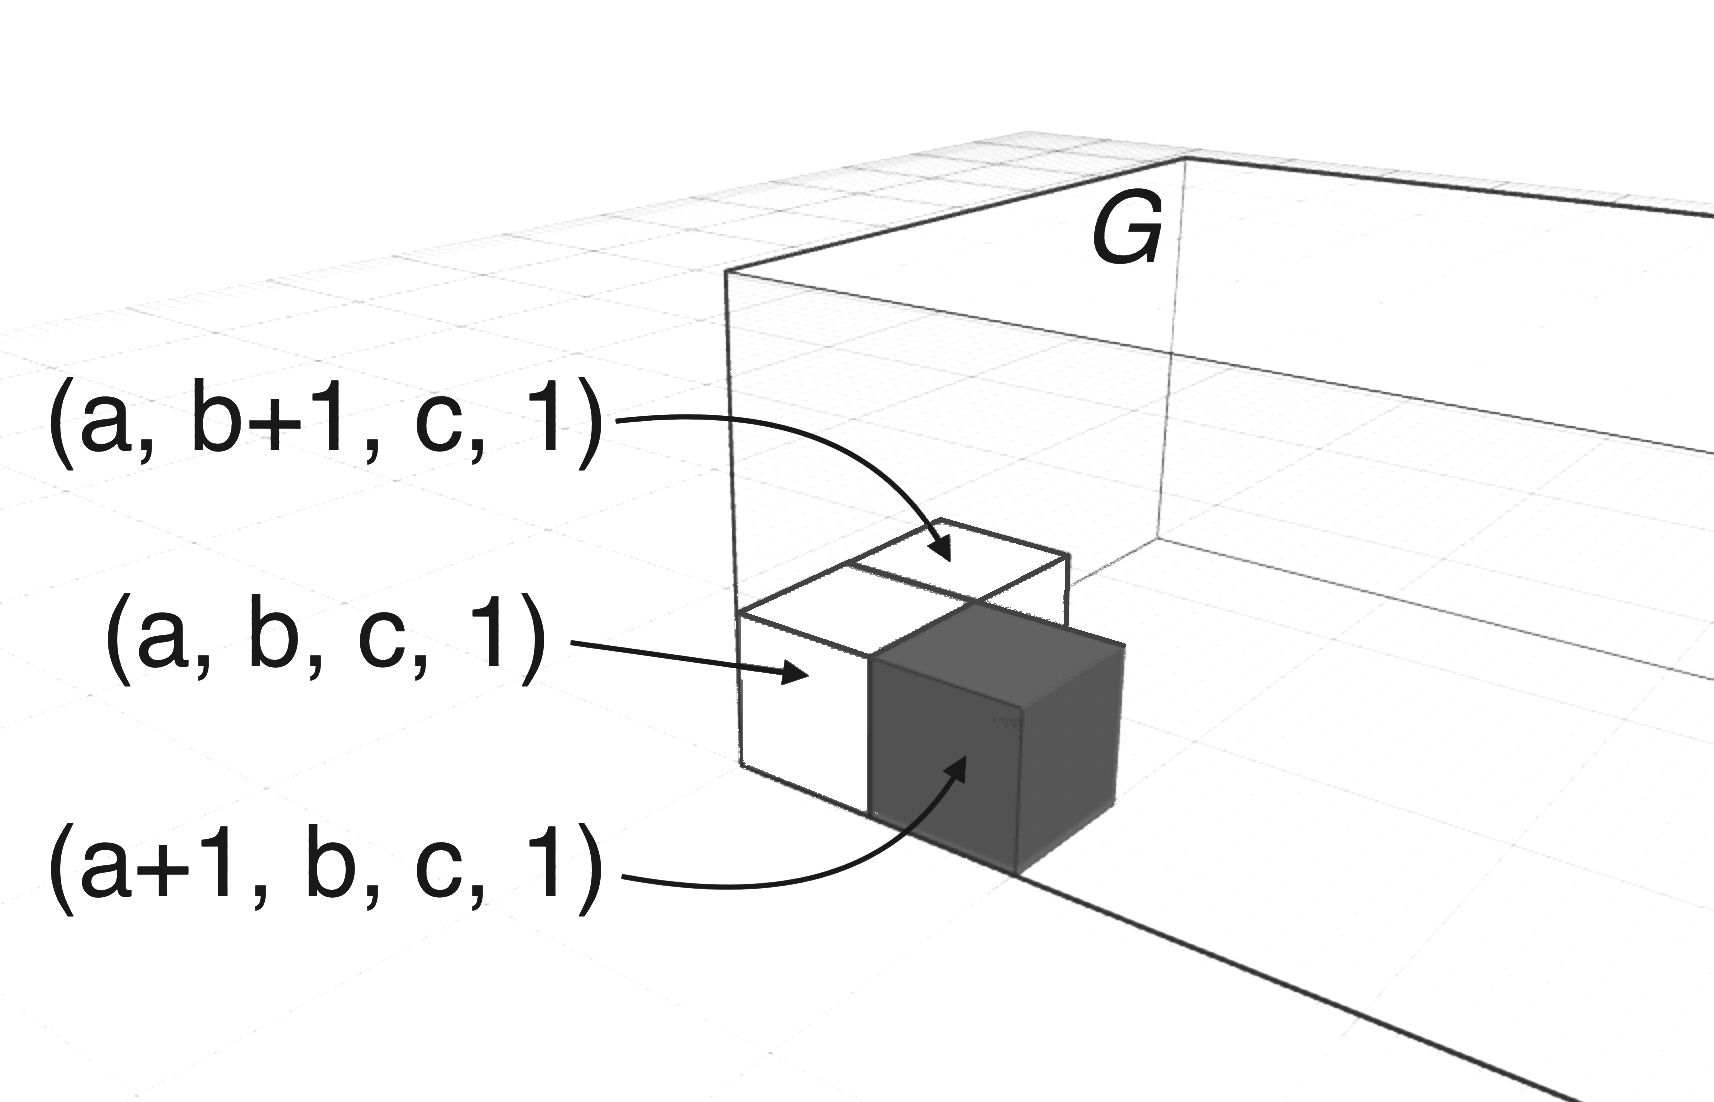
\includegraphics[width=7cm]{nD-G(1).png}
   % \caption{Trodimenziona forma gornjeg sloja četvorodimenzionog kvadra.} 
%\end{figure}

\Figure{nD-G(1).png}{Trodimenziona forma gornjeg sloja četvorodimenzionog kvadra}{Three-dimensional form of the upper layer of the four-dimensional hypercube} 


%\begin{figure}[!h]
 %   \centering
  %  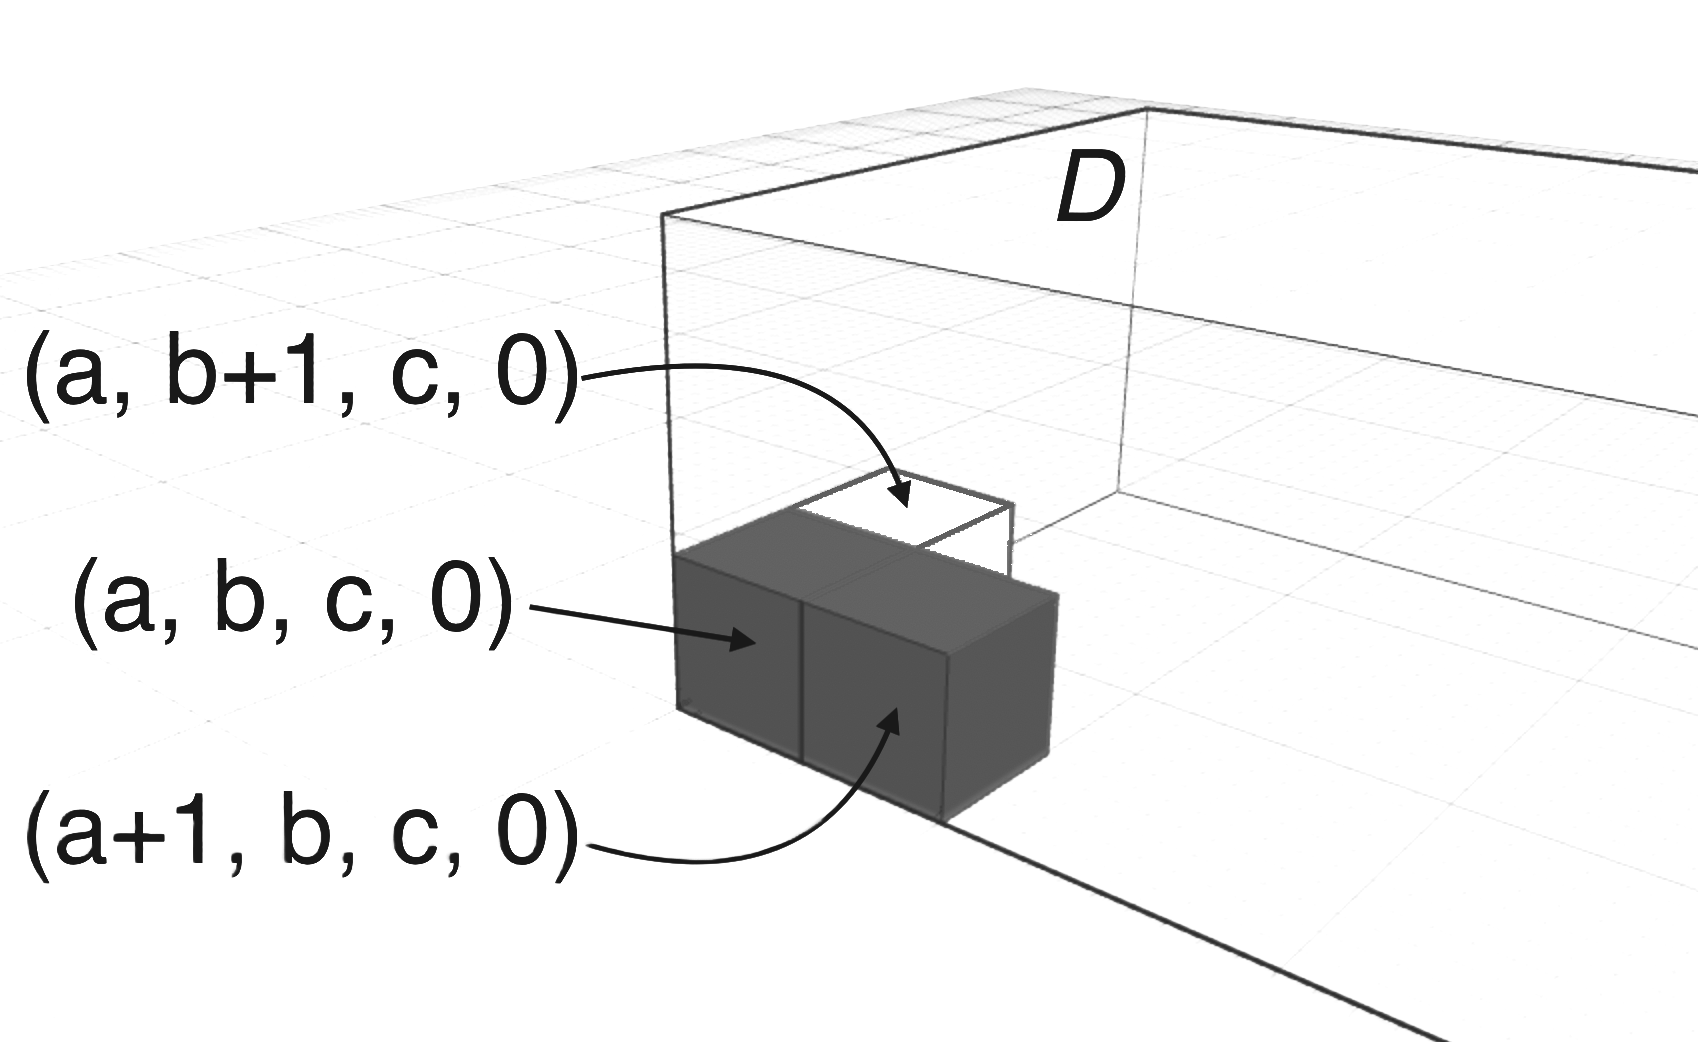
\includegraphics[width=7cm]{nD-D(1).png}
   % \caption{Trodimenziona forma donjeg sloja četvorodimenzionog kvadra.} 
%\end{figure}

\Figure{nD-D(1).png}{Trodimenziona forma donjeg sloja četvorodimenzionog kvadra}{Three-dimensional form of the bottom layer of the four-dimensional hypercube} 

\subsection{Induktivni prelaz}
\begin{Theorem}
    Svaki n-dimenzioni kvadar čija je bar jedna stranica deljiva sa tri i čije su bar dve stranice veće ili jednake sa četiri može se kompaktno popločati n-dimenzionim L-trominama.
\end{Theorem}

%Svaki kvadar $p\times q\times r\times s$ za koji važi $p,q \geq 4$ i $3\mid pqrs$, može se kompaktno popuniti četvorodimenzionim L-trominama.




Dokaz kompaktnog popločavanja n-dimenzionog kvadra se postiže matematičkom indukcijom. Iz prethodnih teorema pokazano je da je rezon podele tela na slojeve jedinične visine koji se kasnije predstavljaju $n-1$ dimenzijom i tako kompaktno popločavaju, ispravan. Matematičkom indukcijom dolazi se do zaključka da se bilo koji problem kompaktnog popločavanja n-dimenzionog kvadra, svođenjem na za jednu manje dimenziju, može svesti na problem kompaktnog popločavanja pravougaonika koji po teoremi 2.7 uvek ima rešenje za pravougaonik za koji važi $p,q \geq 4$ i $3\mid pq$.

\section{Domine}

Domine, kao najpopularnije poliomine su kroz brojne radove temeljno ispitane. Iako su po svojoj prirodi najjednostavnije poliomine i da su rešenja u kojima se one koriste isprva trivijalna, kada je reč o problemima koji uključuju višedimenzione domine, situacija se naglo komplikuje. U ovoj sekciji biće reči o kompaktnim popunjavanjima n-dimenzionog kvadra n-dimenzionim dominama. Koristeći se rezonom iz sekcije o trominama, trodimenziona tromina je telo sačinjeno od dve kocke spojene po jednoj strani. Analogno, n-dimenziona domina je trodimenziona domina kojoj je dodato $n$ dimenzija jedinične vrednosti.

Kao i kod tromina, dokaz kompaktnog popunjavanja n-dimenzionog kvadra će se induktivno izvesti iz dokaza kompaktnog popunjavanja trodimenzionog kvadra L-trominama. Samim time, neophodno je znati koje sve dimenzije slojeva se mogu kompaktno popločati. 

\begin{Theorem}
    Pravougaonik $p\times q$ može se kompaktno popločati pločicama $1\times m$ ako i samo ako su sledeći uslovi ispunjeni:
    \begin{enumerate}
        \item $m\mid p$ ili $m\mid q$
        \item $p,q>2m$ [3]
   \end{enumerate}
\end{Theorem}

\subsection{Domine u 3D}
    


\begin{Theorem}
    Svaki trodimenzioni kvadar $p\times q\times r$, može se kompaktno popuniti dominama ako njegovi slojevi prate uslove Teoreme 6.1, za $m=2$.
\end{Theorem}


Za potrebe dokaza ove teoreme definišemo pojam kritične domine, kao i Leme potrebne za kompletiranje dokaza.

\begin{Definition}
    Kritična domina je domina koja sprečava neku od pravih(ravni) da preseku figuru tj. domina bez koje telo ne bi bilo kompaktno popločano(popunjeno).
\end{Definition}

\begin{Lemma}
    Svaki pravouganik $p\times q$ koji ispunjava uslove teoreme 6.1 ima više od dve domine koje nisu kritične.
\end{Lemma}

\begin{proof}
    Broj pravih koje presecaju pravougonik $p\times q$ tako da mogu narušiti njegovu kompaktnost je $p+q-2$, što znači da kritičnih domina može biti najviše toliko, a ukupan broj domina u tom pravougaoniku je $\frac{pq}{2}$, što znači da je broj domina koje nisu kritične $(p-2)(q-2)$ što je sigurno veće od dva zbog uslova iz Teoreme 6.1.
\end{proof}



\begin{proof}
    Kvadar se deli na slojeve jedinične visine i svaki sloj se popločava zasebno. Kako su ti slojevi pravougaonici dimenzija $p\times q$ izdignuti za jednu jedinicu, za njih je poznato po teoremi 6.1 da se mogu kompaktno poplocati dominama ako je $p,q \geq 5$ i $2\mid pq$.
    Da bi kvadar bio kompaktno popunjen iz uslova kompaktnosti sledi da susedni slojevi moraju biti medjusobno povezani, tacnije mora se pojaviti bar jedna kriticna domina koja ih povezuje.Ta kriticna domina bice formirana tako sto će se izabrati bilo koja domina koja nije kritična u tom sloju i koja je u tom sloju u potpunosti i rotira se za 90 stepeni u smeru ka gornjem sloju tako da jedna  jedinična kocka od kojih je sacinjena ta domina ostana u tom sloju. Tom rotacijom pravi se praznina u donjem sloju ekvivalentan jediničnoj kocki. Da bi se ta praznina popunila na analogan način ćemo rotirati dominu koja se nalazila direktno iznad već rotirane tromine tako da ona popuni prazninu donjeg sloja.(Slika 5)
    Za to nam je potrebno da svaki sloj ima bar dve kritične domina, a to važi na osnovu Leme.
    Kako sada znamo da uvek mžemo da izaberemo dominu koja će postati kritična to znači da možemo spojiti bilo koji broj slojeva međusobno, što znači da ta dimenzija ne utiče na to da li se kvadar može kompaktno popuniti, a i samim tim da je jedini uslov koji je potreban da bi se kvadar mogao kompaktno popuniti ustvari da dve njegove dimenzije zadovoljavaju uslove Teoreme 6.1, čime je dokaz završen. 
\end{proof}

\subsection{Domine u nD}

\begin{Theorem}
    Svaki n-dimenzioni kvadar sa slojevima koji ispunjavaju uslove teoreme 6.2 može se kompaktno popločati n-dimenzionim dominama.
\end{Theorem}

Rezoн dokaza kompaktnog popunjavanja n-dimenzionog kvadra n-dimenzionim dominama je 
identičan koa kod kompaktnog popunjavanja n-dimenzionog kvadra n-dimenzionim L-trominama. Budući da je poznat dokaz kompaktnog popunjavanja trodimenzionog kvadra, ponovo se problem kompaktnog popunjavanja svodi na problem manje dimenzije. Prvo se četvorodimenzioni kvadar podeli na četvorodimenzione slojeve jedinične četvorodimenzione visine. Zbog jedinične četvorodimenzione visine, dobijeni slojevi se mogu posmatrati kao trodimenzioni objekti. Po teoremi 6.1 ovi slojevi se mogu kompaktno popločati. Spajanje dva sloja takođe funkcioniše na dosda već poznat način. 

Budući da su slojevi zapravo četvorodienzioni oblici koji su zbog jedinične četvorodimenzione visine predstavljeni kao trodimenzione figure, kada se slojevi spoje u četvrtoj dimenziji, zajedno sa njima će i domine koje formiraju spajajuću konfiguraciju postati tridimensional, spajajući dva sloja četvorodimenzionog kvadra.

Dokaz kompaktnog popločavanja n-dimenzionog kvadra se postiže matematičkom indukcijom na isti način kao i kod kompaktnog popunjavanja n-dimenzionog kvadra n-dimenzionim L-trominama.


\section{Prebrojavanje}

%Kada se telo kompaktno poploča nekom figurom, to se smatra jednim od kompaktnih popločavanja, ali to nije jedino popločavanje moguće. Postavlja se pitanje na koliko načina se može neki pravougaonik popločati L-trominama.

Intuitivno je pretpostaviti da oblicic koji se mogu kompaktno popločati poseduju više pd jednog načina popločavanja. Prirodno je postaviti pitanje na koliko različitih načina se neki oblik može kompaktno popločati. Jedan problem slične tematike je već rešen. Naime, postoji formula koja opisuje broj različitih kompaktnih popločavanja pravouganik $2m\times 2n$ sa $2mn$. Formula je sledeće:


    $$4^{mn} \prod_{j=1}^{m} \prod_{k=1}^{n} \left\{ \cos^2 \left( \frac{j\pi}{2m+1} \right) + \cos^2 \left( \frac{k\pi}{2n+1} \right) \right\}$$ 

Budući da je ova formula pomalo zastrašujuća i uzimajući u obzir kompleksnost prebrojavanja kompaktnih popločavanja L-trominama, procenili smo da je prebrojavanje različitih kompaktnih popločavanje dvodimenzionih tela prekomlikovano. Samim time, u ovom radu biće reči o postavljanju donje granice za broj različitih kompaktnih popunjavanja trodimenzionog kvadra. 

Naime, razmatraćemo samo slučajeve gde se trodimenzioni kvadar sastoji iz identično popločanih slojeva. Ovo nam omogućava da prebrojavamo samo broj različitih povezivanja dva sloja jednom kofiguracijom spajanja bez osvrtanja na ostale konfiguracije. Potrebno je takođe obratiti pažnju na tromine koje se koriste za povezivanje. Recimo, tromine iz drugog sloja koje su se koristile za povezivanje prvog i drugog sloja, ne mogu se koristiti za povezivanje drugog i trećeg sloja. 

Data formula predstavlja donju granicu različitih kompaktnih popunjavanja trodimenzionog kvadra trodimenzionim L-trominama gde $S$ predstavlja broj slobodnih (nekritičnih) tromina podobne za povezivane neka dva sloja:

\[
\sum_{(i_1, \dots, i_{n-1}) \in \mathbb{N}^{n-1}} \prod_{k=1}^{n-1} \binom{s - i_{k-1}}{i_k}
\]
gde $i_{k} + i_{k+1} \le S, k=1,2..n-1$.
Logika iza dobijene formule jeste da binomne formule označavaju broj načina na koji se slobodne tromine mogu izabrati i da u svakom sleddećem sloju slobodne tromine koje su prethodno izabrane ne mogu se u narednom sloju birati, jer su već rotirane, ali već u narednom ih je moguće opet birati kao slobodne(gde notacija slobodne tromine označava L-trominu koja nije kritična)
%ekstremno neformalno je ali jbg%



\section{Pravci za dalji rad}

Dalji rad ćemo posvetiti primarno problemu prebrojavanja gde ćemo gledati nakoliko načina se može neki pravouganok popločati L-trominama i tu ćemu gledati da možda dobijemo neku konkretnu formulu, kao što je dobijeno kod domina, ali je proces mnogo složeniji, jer kod domina postoji mali broj načina na koji se one mogu uklopiti dok je kod L-tromina veći broj, pa se samim tim dosta komplikuje.

Gledaćemo da možda i vidimo prebrojavanje mogućih popunjavanja kvadra, ali tu je isto proces zahtevan jer se kritična tromina može izabrati na dosta načina, ali bi sa druge strane trebalo da se ponovi isti proces posle konačnog broja izdizanja, pa bi smo tu verovatno gledali da damu neku gornju granicu.


\section{Zaključak}

Cilj projekta bio je da posmatramo raznorazna popločavanja i popunjavanja L-tromina, jer su ona bila potpuno neistražena, pogotovo u višedimenzionim prostorima. Rezultati koje smo dobili u 2D smo osmislili intuitivno i bili su nam osnova za celokupan rad. Bitno je napomenuti da većina ovih dokazanih stvari izvodi se poprilično analogno za domine, u nekim slučajevima čak i jednostavnije.


\section{Literatura}
\Source{
    Mridul Aanjaneya \& Sudebkumar Prasant (2006): Faultfree Tromino Tilings of Rectangles, arXiv: Combinatorics, math/0610925
}
\Source{
    Solomon W. Golomb (2020):  Polyominoes: Puzzles, Patterns, Problems, and Packings - Revised and Expanded Second Edition, Princeton University Press
}
\Source{
    Norton Starr (2008): Tromino Tiling Deficient Cubes of Any Side Length, arXiv: Combinatorics, math/0806.0524
}
\Source{
    Herman Tulleken (2018): Polyominoes, ResearchGate manuscript
}

\EndPaper

